\subsection{Overlaping to Hide Latency}



\begin{figure}
  \centering
    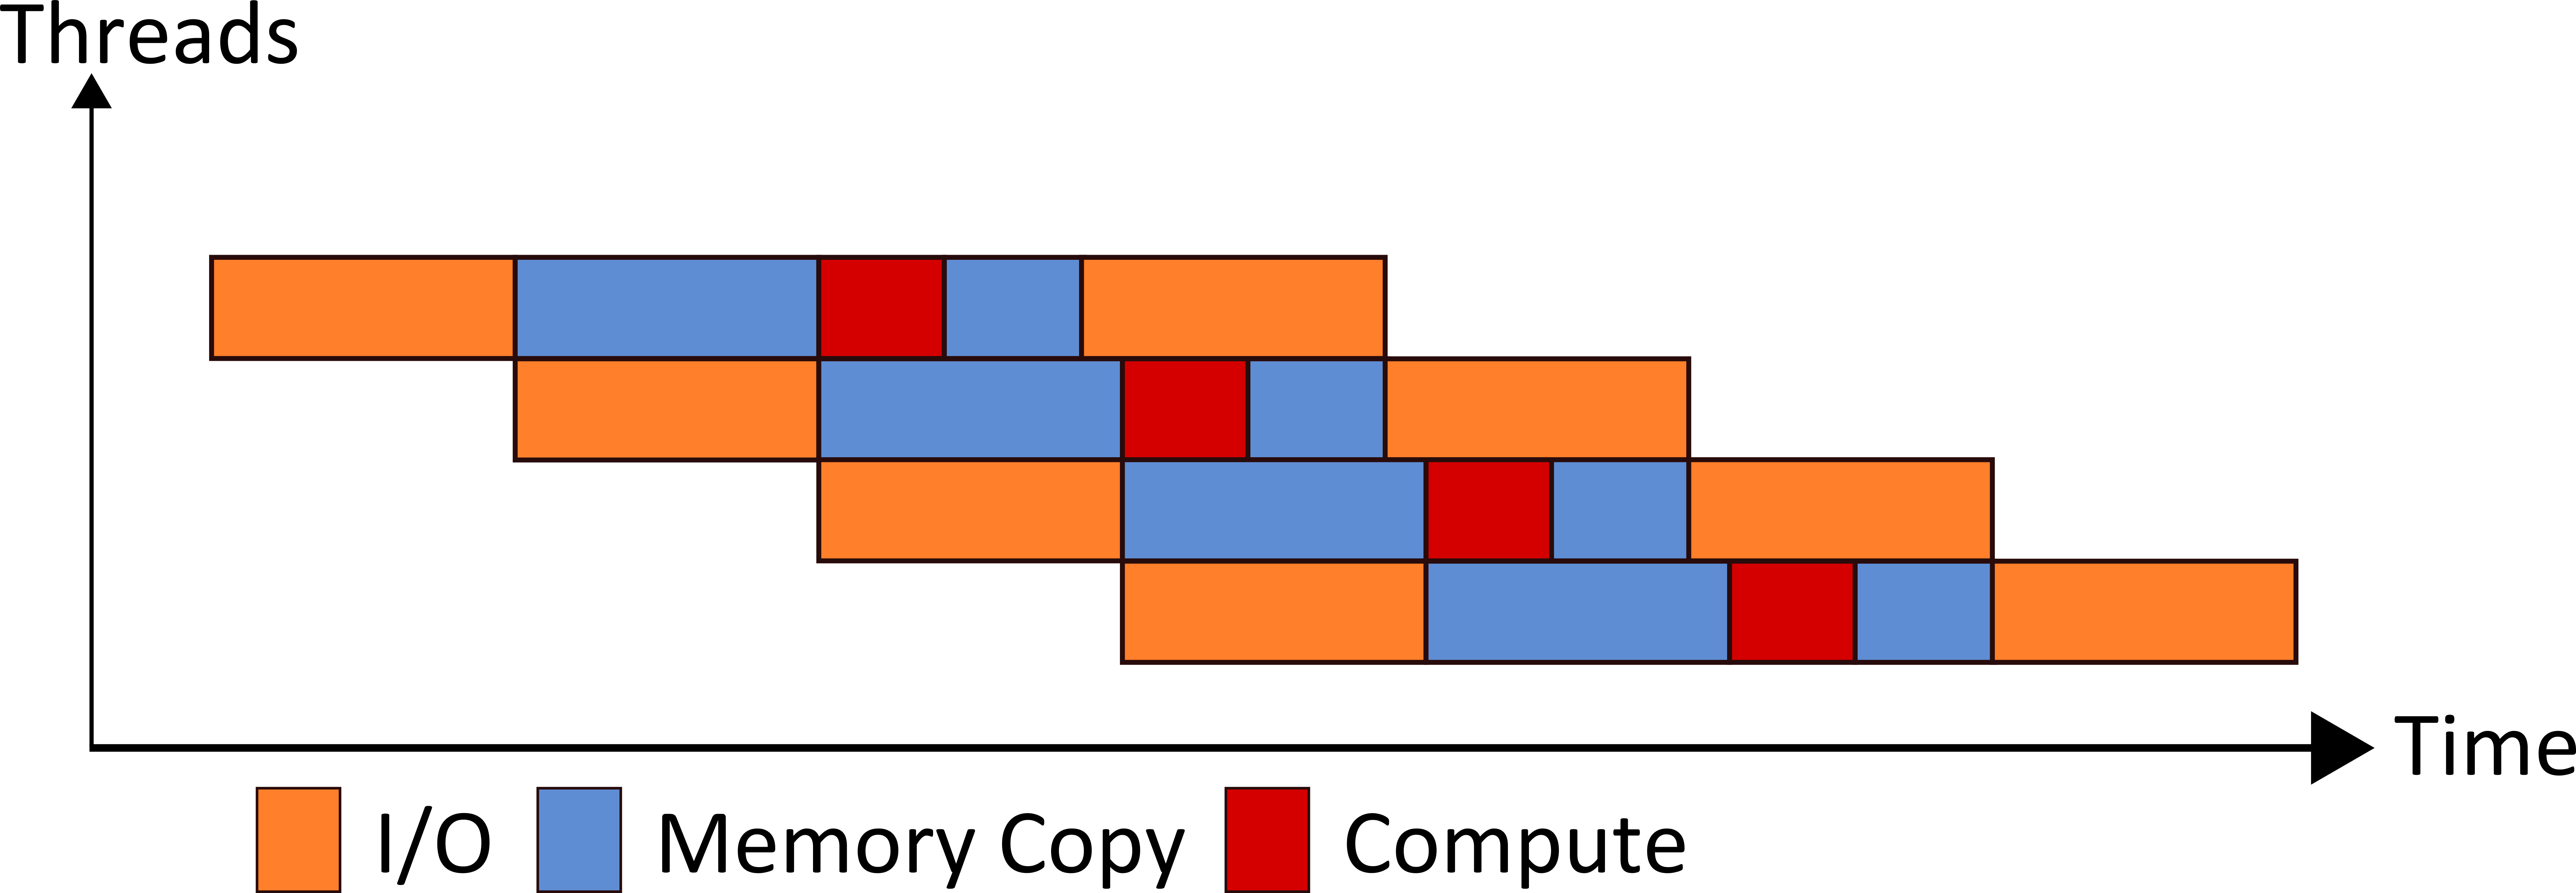
\includegraphics[width=0.5\textwidth]{fig/ord.png}
  \caption{A representation of simple overlap of host I/O, host-to-device data
           transfer, and kernel execution. In this example, there are no
           dependencies between kernels and data so management is relateively
           simple.}
  \label{fig:unord}
\end{figure}

\begin{figure}
  \centering
    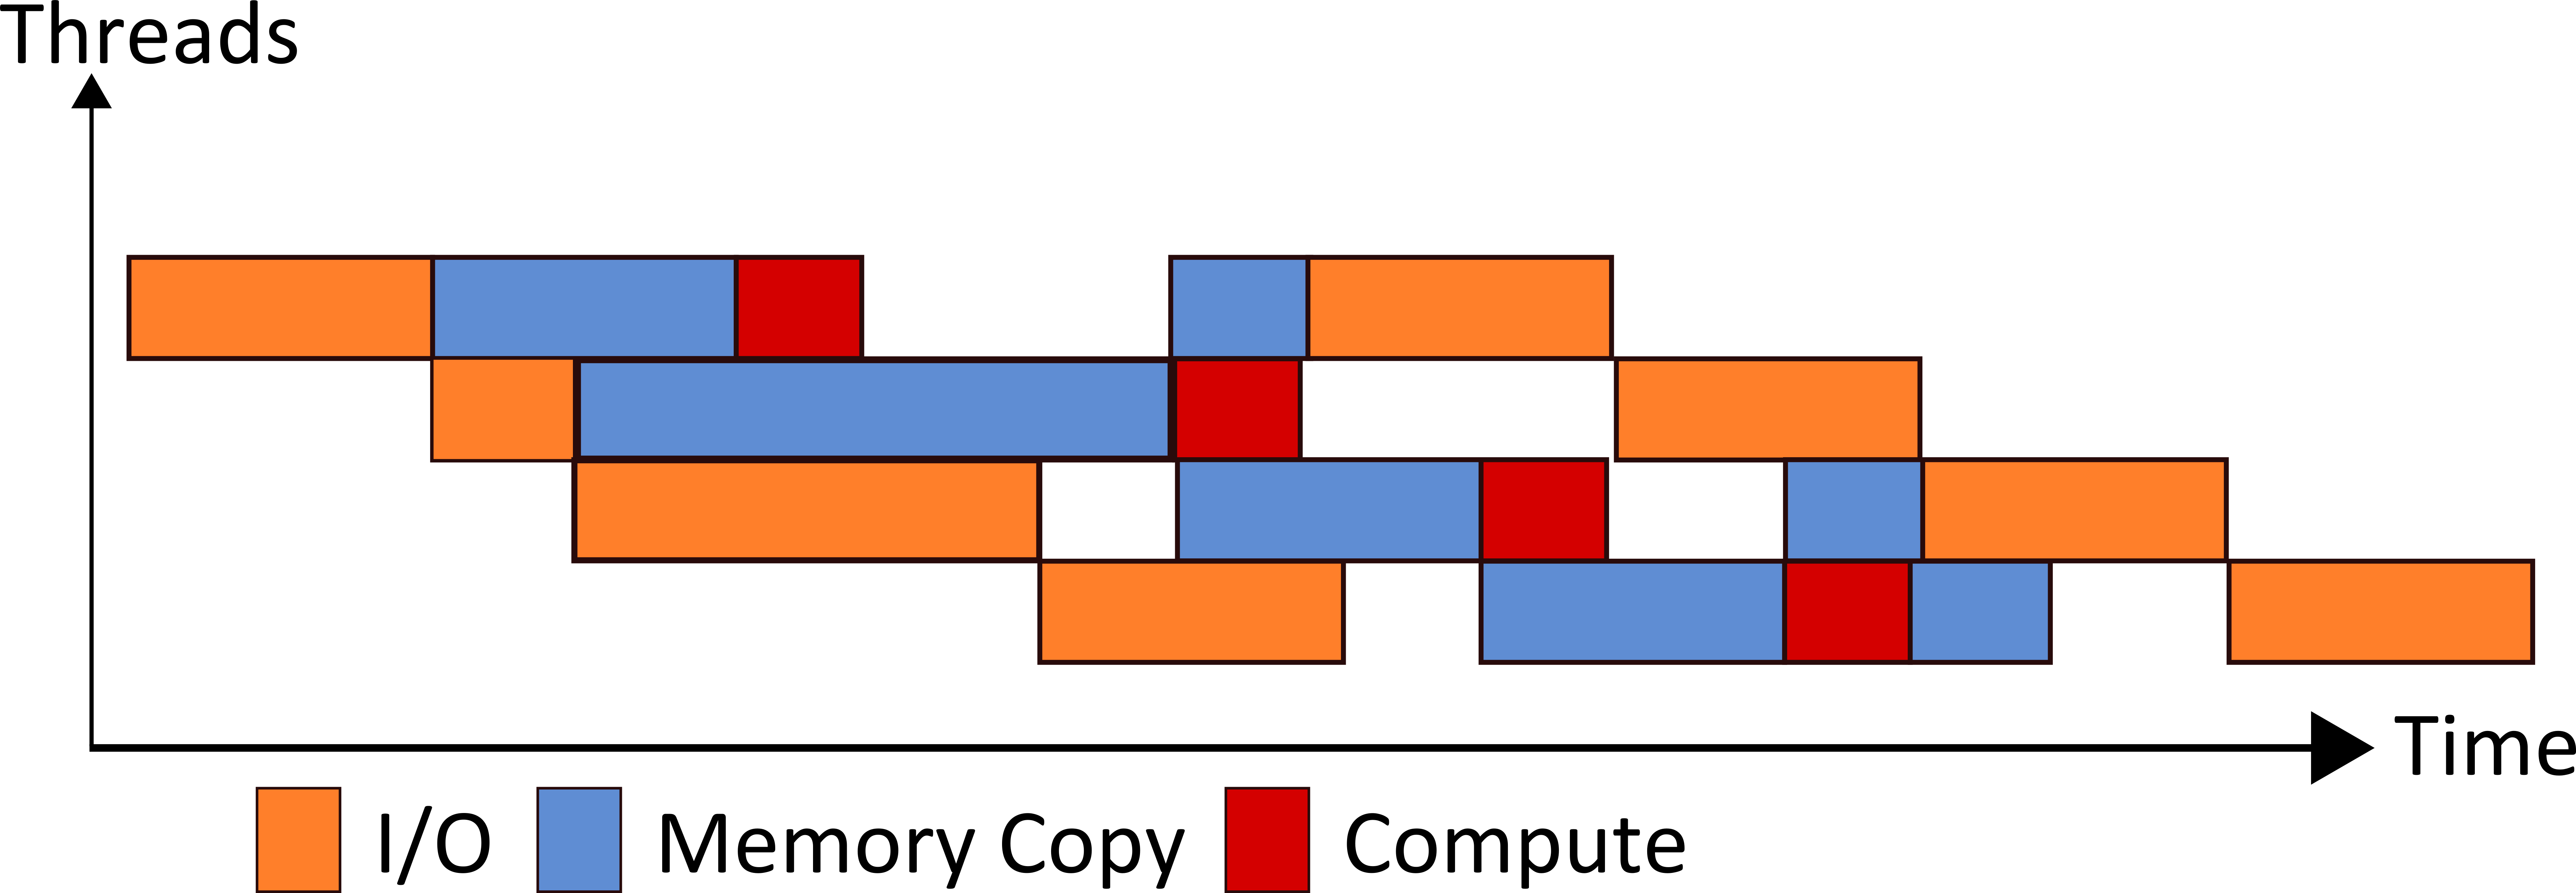
\includegraphics[width=0.5\textwidth]{fig/unord.png}
  \caption{A more complicated oververlap of host I/O, host-to-device data
           transfer, and kernel execution. Arbitrary data-dependence between
           kernels and transfers places too large a burden on the programmer
           to manage properly.}
  \label{fig:unord}
\end{figure}

In many cases certain overlapings are not possible, either because of
  hardware restrictions or language semantic restrictions.
In CUDA, for example, two copy memory to device operations cannot be
overlapped since they both share the same PCI-Express bus.
One can overlap the compute with the copy memory to device, however.
This results in the programer having to add logic to keep track of which
  overlaps are occuring at which point --- causing the program to be
  more complicated.
This is show in figure~\ref{fig:unord}.

 

